\chapter{Implementación del sistema operativo}

Una vez que sabemos las decisiones tomadas y las tecnologías utilizadas, pasemos a estudiar cada una de las soluciones implementadas en confrontación con los requisitos estudiados.\\

Empezaremos por la puesta a punto del sistema de compilación y continuaremos con la configuración necesaria para el funcionamiento esperado del sistema operativo embebido. Dado el volumen del proyecto \textit{Yocto}, describiremos solo parcialmente sus factores de configuración y el proceso de trabajo con él.

\section{Introducción y puesta a punto}

Como venimos mencionando a lo largo de la memoria, el proyecto \textit{Yocto} se basa en la herramienta \textit{Open Embedded} y en el lenguaje de configuración \textit{Bitbake}, que permite ajustar desde parámetros del \textit{kernel} hasta elegir paquetes que no se quiere sean instalados. Además, cabe destacar que se pueden compilar imágenes con \textit{Yocto} de diversas formas, ya sea utilizando contenedores aislados (a modo de máquinas virtuales) o nuestro propio sistema \textit{Linux} \textit{anfitrión}, como vemos en la documentación de inicio \cite{yocto-project-quick-start-build-system}. Por mi parte, siempre he preferido hacerlo en el propio sistema, dado que así se destinan a la compilación el 100\% de los recursos asignados disponibles y el tiempo de espera es menor.\\

Para el caso que nos ocupa, la versión utilizada del proyecto \textit{Yocto} ha sido la \textbf{2.4} (de nombre \textit{Rocko}), dado que se trataba de la versión estable más avanzada en el momento del desarrollo.\\

La guía relativa a la puesta a punto la encontramos en el manual \textit{Quick Start} de la web \cite{yocto-project-quick-start} ya mencionado, y consiste principalmente en instalar las dependencias necesarias para nuestra distribución y clonar mediante \texttt{git} el núcleo del proyecto, llamado \textit{Poky}, con el comando siguiente (la opción \texttt{-b} elige la rama deseada):

\begin{center}
\texttt{git clone git://git.yoctoproject.org/poky -b rocko}
\end{center}

\subsection{Manipulación y compilación de prueba}

Una vez tenemos el núcleo, lo siguiente es empezar a configurar el resultado que queremos obtener. Si ejecutamos el comando \texttt{source oe-init-build-env}, se nos generará un directorio destino \textit{build} con una configuración de ejemplo para una máquina \textit{Qemu} de 32 bits.\\ 

La premisa de este tipo de sistemas de desarrollo es incluir lo mínimo para funcionar, y que sea el desarrollador quien elija las dependencias a incluir. Por tanto, aunque dicho archivo de configuración es grande, se trata de mucho código de ejemplo y comentarios de ayuda al recién llegado.\\

Aquí podemos elegir entre cambiar el dispositivo de destino y los paquetes a instalar, o seguir adelante con una imagen mínima de prueba de la siguiente forma:

\begin{center}
\texttt{bitbake core-image-minimal}
\end{center}

El nombre \texttt{core-image-minimal} hace referencia a la imagen de menor tamaño por defecto, por lo que para hacer pruebas es suficiente. \\

Habremos de esperar un tiempo de entre treinta minutos y dos horas aproximadamente a que se descarguen todos los paquetes necesarios y se compilen. Tras esto, se habrá generado un archivo de imagen con extensión \textit{.sdimg} en el directorio \textit{./build/tmp/deploy/images/raspberrypi3/}.\\

Podremos \textit{quemar} (o instalar) esta imagen en una tarjeta de memoria con la conocida utilidad \textit{dd}, presente en cualquier sistema \textit{GNU/Linux}, siendo \texttt{/dev/sdX} el dispositivo referente a la tarjeta de memoria:\\

\texttt{sudo dd if=core-image-minimal-raspberrypi3.sdimg of=/dev/sdX}\\

Acto seguido podremos insertar la tarjeta de memoria en la placa y encenderla para entrar en el sistema.

\subsection{Variables de configuración del sistema}

La sintaxis de configuración es sencilla, y sigue la forma: 

\begin{center}
	\texttt{PARÁMETRO\_CONFIGURACIÓN = "valor deseado"}
\end{center}

En el directorio \textit{build} antes creado, podremos ir incorporando configuración al archivo \texttt{conf/local.conf} con dicha sintaxis de la herramienta \textit{Bitbake} para instalar/borrar paquetes del dispositivo.\\

La sintaxis de código para añadir dependencias sería la siguiente (hemos de añadir esta línea al archivo \textit{conf/local.conf} mencionado):

\begin{center}
\texttt{IMAGE\_INSTALL\_append = `` <paquete1> <paquete2> ...''}
\end{center}

Si quisiéramos eliminar alguno de los paquetes incluidos por alguna librería necesaria, es tan fácil como sustituir \texttt{append} por \texttt{remove}.\\

Por otro lado, si profundizamos en los archivos de configuración descargados de cualquiera de los \textit{layers}, encontramos en alguna ocasión configuración de la forma:

\begin{center}
\texttt{VARIABLE ?= "valor"}
\end{center}

Cuando un símbolo de interrogación acompaña a esta variable, significa que es un \textbf{valor por defecto}, fácilmente anulable por una asignación sin dicho símbolo en cualquier parte.\\

Por ejemplo, en la configuración por defecto, el dispositivo por destino se muestra tal que así:

\begin{center}
\texttt{MACHINE ?= "qemux86"}
\end{center}

En nuestro caso, borraremos la interrogación y escribiremos ``raspberrypi3'' entre comillas, dado que es nuestro dispositivo elegido (podemos consultar el listado completo en \href{http://layers.openembedded.org/layerindex/branch/master/machines/?q=&browse=1}{\textit{OpenEmbedded Layer Index}}, junto con los \textit{layers} necesarios para cada máquina).\\

\subsection{\textit{Layers} y librerías}

Por otro lado, la forma de reutilizar librerías y \textit{layers} ya existentes es sencilla. Podemos encontrar la lista completa de \textit{layers} y paquetes pertenecientes a éstas en la referencia \cite{yocto-layers-list}. Para empezar basta con descargarlas (también mediante \texttt{git}) en el directorio raíz del sistema de compilación. Acto seguido, añadimos una línea en el fichero \texttt{./build/conf/bblayers.conf} con la ruta a la librería descargada. [\textit{bblayers} toma su nombre por \textit{Bitbake Layers}.] Hecho esto, el comando \texttt{bitbake} detectará todos los paquetes y dependencias que tenemos importados en el sistema, viéndose esto reflejado en cada compilación.\\

En la web antes mencionada, \url{https://layers.openembedded.org}, dentro de la sección \textbf{\textit{Recipes}} podemos buscar paquetes que nos interesen, dando con la(s) capa(s) que los incluyen. Por ejemplo, si quisiéramos utilizar \textit{PSplash}, una herramienta para imprimir imágenes de carga embebidas, obtendríamos lo siguiente:

\begin{figure}[H]
	\centering
	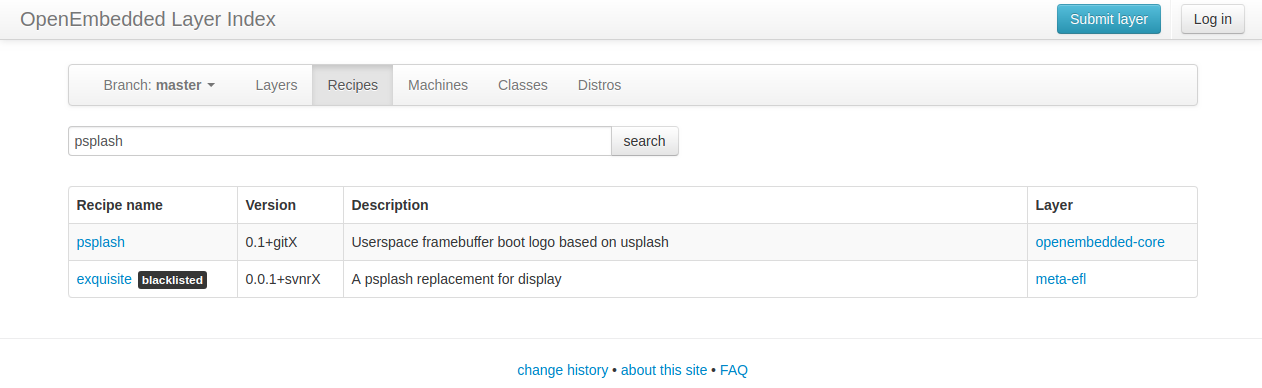
\includegraphics[width=\linewidth]{imagenes/yocto-recipe-search-example.png}
	\caption{Ejemplo de búsqueda en las recetas de \textit{OpenEmbedded} [13/06/2018]}
	\label{yocto-recipe-search-example}
\end{figure}

Como vemos, los resultados vienen compuestos del nombre de los paquetes, las versiones (para filtrar cuando existen varias del mismo), una descripción inteligible y el \textit{layer} donde encontrarlo. Si hacemos \textit{click} en el nombre del \textit{layer}, veremos una descripción de dicho layer y la dirección del repositorio donde se aloja (y que habremos de clonar).\\

\subsubsection{\textit{Layer} propio}

Como aconsejan en la propia documentación de \textit{Yocto}, una vez que queremos pasar de hacer pruebas a confeccionar nuestro producto, lo idóneo es \textbf{crear un \textit{layer} propio} en el que alojar la configuración de forma aislada. Por ejemplo, en nuestro caso la capa usada recibe el nombre de \texttt{meta-dynasystem} y da nombre a este proyecto.\\

Los pasos para crear un \textit{layer}, descritos en la propia \textit{Wiki} de \textit{Yocto} \cite{wiki-yocto-own-layer}, son sencillos. El proceso consiste básicamente en generar un par de carpetas y un archivo de configuración común al \textit{layer} (llamado \texttt{layer.conf}), describiendo las rutas internas al \textit{layer} y la prioridad de sus paquetes con respecto a los de otras.\\

Por otro lado, debemos saber que dentro de cada \textit{layer} existirán distintos subniveles de directorios: 

\begin{itemize}
	\item \textbf{Configuración propia del layer \texttt{(/conf)}}: el archivo necesario se aloja en la ruta antes mencionada \texttt{./conf/layer.conf}.
	\item \textbf{Ficheros de clases \texttt{(/classes)}}: las clases representan comportamientos específicos que pueden heredar las imágenes de sistema. Tienen extensión \texttt{.bbclass}.
	\item \textbf{Recetas de paquetes de todo tipo \texttt{(/recipes-X)}}: siendo ``X'' variable y reflejando el tipo de las recetas que se usan. Por ejemplo, los paquetes importantes o las imágenes suelen ser incluidas en una carpeta llamada \textbf{\textit{recipes-core}}; o las recetas relacionadas con Mender se agrupan en la carpeta \textbf{\textit{recipes-mender}}.
\end{itemize}

Dentro de estas carpetas de recetas encontraremos un directorio por cada paquete de la categoría. Comentemos esto en el siguiente apartado.\\

\subsection{Paquetes, configuración y parches}

Como hemos dicho anteriormente, encontramos una carpeta para cada paquete existente, con el mismo nombre del paquete. De forma interna a esta, podremos distinguir varios subdirectorios y archivos:

\begin{itemize}
	\item \textbf{Archivos a incluir en el sistema \texttt{(/files)}}: aquí se alojan ficheros de todo tipo que se quiere figuren en el sistema final asociados al paquete (scrips, documentos, etc.).
	\item \textbf{Parches por aplicar al paquete \texttt{(/patches)}}: comentaremos su función de forma más extensa en esta sección más adelante.
	\item \textbf{Configuración adicional para el paquete \texttt{(paquete\_\%.bbappend)}}: <paquete> se refiere al nombre, y ``\%'' simboliza el número de versión. En este archivo se hace referencia a los ficheros del directorio \texttt{/files} y los parches de \texttt{/patches} que se quieren tomar en consideración.
\end{itemize}

Para terminar con la introducción a \textit{Yocto}, cabe destacar la importancia de \textbf{los parches} previamente mencionados (o \textit{patches} en inglés). Estos permitirán de una forma escalable y, sobre todo automatizada, modificar el comportamiento de las aplicaciones y programas libres ya presentes en los repositorios.\\

Para entender el funcionamiento de los parches, veamos antes los estados por los que pasa un paquete por compilar:

\begin{enumerate}
	\item Se descarga el código fuente de la aplicación. El repositorio desde el que se descarga vendrá especificado por el fichero \textbf{\textit{``receta.bb''}} propio del paquete. Por ejemplo, la receta del paquete \textit{PSplash} \cite{yocto-recipe-psplash}. La variable que almacena el enlace se llama \texttt{SRC\_URI}.
	\item Los \textit{layers} pueden aplicar configuración y parches al código descargado de otros \textit{layers}, guardando estas modificaciones en archivos \textbf{\textit{``receta.bbappend''}}. Después del primer paso, para cada paquete se buscan todos los ficheros \textit{.bbappend} que le correspondan, y se aplican las modificaciones oportunas.
	\item Una vez aplicados todos los parches, se compila el código completo y se incluye para ser instalado en la imagen de destino.
\end{enumerate}

Esto representado en \textit{UML} en forma de diagrama de estados sería tal que así:

\begin{figure}[H]
	\centering
	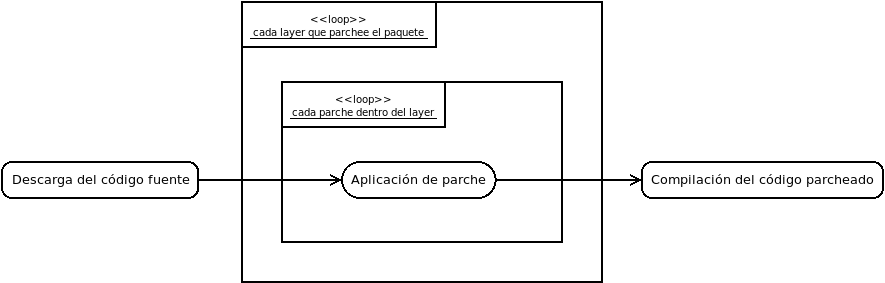
\includegraphics[width=\linewidth]{imagenes/statechart-parche.png}
	\caption{Diagrama de estados por los que pasa una dependencia en \textit{Open Embedded}}
	\label{statechart-parche}
\end{figure}

\noindent\makebox[\linewidth]{\rule{\textwidth}{0.4pt}}\\

\subsubsection{Proceso de parcheo de paquetes}

Por otro lado, un recién llegado al proyecto podría pensar que la forma de redefinir comportamientos en paquetes ya existentes consiste en:

\begin{enumerate}
	\item Hacer en otro repositorio un \textit{fork} del programa en cuestión.
	\item Realizar las modificaciones pertinentes de forma aislada.
	\item Crear una receta en \textit{Yocto} que obtenga el paquete desde el nuevo repositorio, con prioridad mayor al original.
\end{enumerate}

Yo mismo probé a hacerlo durante un tiempo, pero a pesar de que esto realmente puede llegar a ``funcionar'', es desacertado, pues además de ser lento y arduo no aporta escalabilidad ni automatización de ningún tipo.\\

La forma escalable de trabajar viene dada por \textbf{la herramienta \textit{devtool}}, que genera una copia local del código fuente del programa listo para que realicemos las modificaciones pertinentes. Además, nos permitirá realizar compilaciones utilizando esta versión temporal, para verificar el funcionamiento de los cambios añadidos. Encontramos la guía de estos pasos en la referencia \cite{wiki-yocto-patches}.\\

Ejecutamos \texttt{devtool nombre\_del\_paquete} y la herramienta descargará el código fuente, le serán aplicados todos los parches de los \textit{layers} existentes por parte de \textit{bitbake}, y será generada una carpeta \texttt{./build/tmp/sources/nombre\_del\_paquete} con este código final.\\

Sobre el código de este directorio será sobre el que hagamos las modificaciones. Para probar estos cambios, bastará con compilar el paquete de forma aislada (\texttt{bitbake nombre\_del\_paquete}) y ejecutarlo.\\

\subsubsection{Inclusión de parches en \textit{layer} propio}

Cuando terminemos con las pruebas y queramos guardar los cambios realizados, deberemos generar un archivo en forma de parche interpretable de forma automática por \textit{Bitbake}, y que quede de forma persistente en nuestro propio \textit{layer}.\\

\textit{Bitbake} detectará automáticamente la existencia de estos parches y los aplicará al código fuente del programa antes de compilarlo e instalarlo en la imagen de destino. Para desarrollar sistemas con \textit{Yocto}, es una de las mecánicas más usadas, ya que generalmente existen paquetes para casi cualquier necesidad que tengamos, pero siempre están abiertos a modificaciones más especiales.\\

El comando de generación de parches es simple y conocido, dado que no es específico de \textit{Bitbake} sino de \textit{GNU/Linux}. Para el caso de un parche a un paquete genérico, el comando tendría la siguiente estructura:\\

\textit{\textbf{git diff ./build/tmp/sources/<paquete>/<fichero\_modificado> \\./<layer\_propio>/recipes-<X>/patches/<paquete>.patch}}\\

\noindent\makebox[\linewidth]{\rule{\textwidth}{0.4pt}}\\

Una vez que tenemos el parche generado e importado en nuestro \textit{layer}, necesitaremos hacer ver a la receta original del paquete parcheado la existencia de dichas modificaciones. Para ello crearemos una receta del tipo \textit{.bbappend} como las ya antes mencionadas, con el siguiente contenido:

\begin{lstlisting}
FILESEXTRAPATHS_prepend := "${THISDIR}/patches:"
\end{lstlisting}

Esto provocará que \textit{Bitbake} automáticamente tenga en cuenta estos cambios y los incorpore sobre el código original del paquete.\\

Una vez hayamos hecho esto, podremos centrarnos en los paquetes utilizados y/o desarrollados para satisfacer las necesidades del producto.

\section{Desarrollo de los paquetes necesarios}

Una vez que tenemos una ligera idea de cómo funciona el entorno de trabajo de \textit{Open Embedded/Yocto Project} nos será más sencillo entender las soluciones implementadas para satisfacer los requisitos estudiados.\\

Empezaremos por generar una imagen para un sistema mínimo, sobre la que iremos añadiendo dependencias que satisfagan dichos requerimientos (funcionales o no funcionales).

\subsection{Sistema mínimo}

El archivo con la configuración final del sistema se encuentra en \texttt{dynasystem-image} \cite{dynasystem-image}, aunque la configuración mínima para funcionar sería, además de lo comentado en \textit{./build/conf/local.conf}, lo siguiente:\\

\texttt{\# dynasystem-image\\
inherit core-image\\
IMAGE\_INSTALL += "packagegroup-core-boot"\\
IMAGE\_FEATURES += "ssh-server-dropbear"}\\

-- El nombre \texttt{core-image} hace referencia a la clase mínima necesaria para cualquier imagen de \textit{Yocto}. De esta toma las bases para entenderse como imagen final de dispositivo y las referencias para ser compilada de forma exitosa.\\

-- Con la segunda línea hacemos referencia a todo el grupo de paquetes necesarios para arrancar una máquina con los paquetes mínimos necesarios.\\

-- Por último, instalamos la característica del servidor \textit{SSH} para administrar de forma fácil el sistema.\\

Una vez que tenemos esta configuración guardada en el fichero \textit{./meta-dyna-system/recipes-core/images/dynasystem-image.bb}, basta con compilar la imagen con la orden: \texttt{bitbake dynasystem-image}.\\

En este punto la distribución no aporta gran cosa, ya que lo único que hace es cargar el \textit{kernel} sin apenas programas instalados. Para dotarle de funcionalidades, necesitaremos ver la siguiente sección.

\subsection{Soluciones implementadas/usadas}

Con los apartados comentados previamente, ya disponemos de un sistema capaz de arrancar en modo terminal de comandos. Sin embargo, no permite hacer \textit{nada} más, por lo que serán necesarias labores de implementación y reutilización de código para dotar al sistema de las características requeridas:

\subsubsection{Arranque rápido del sistema}

Por defecto, la imagen mínima del sistema utiliza \textit{\textbf{sysvinit}} como gestor de arranque; un motor antiguo pero estable. Sin embargo, según las pruebas realizadas en los inicios del proyecto, demoraba el inicio del dispositivo en \textbf{unos 45-50 segundos}. Para un sistema tan ligero, no tendría sentido sufrir esta latencia.\\

Este retraso se debe a que el sistema operativo no pasa a estar completamente funcional hasta que no están cargados todos y cada uno de los componentes del sistema operativo.\\

Dada mi experiencia con las distintas distribuciones de \textit{GNU/Linux} y sus gestores de arranque, me animé a probar a integrar \textit{\textbf{systemd}} a modo de motor, dado que se trata de una alternativa más novedosa, basada en servicios independientes que se cargan sucesivamente en segundo plano con el núcleo ya cargado y funcionando.\\

Además, \textit{systemd} ofrece una manera muy intuitiva de creación y administración de servicios. Gracias a esto, es posible crear un nuevo fichero \texttt{<programa>.service} que gestione cuándo debe ser lanzado un programa. Esto facilita la iniciación automática de dependencias del sistema, como veremos más adelante.\\

Para tomar \textit{systemd} como gestor de arranque predeterminado, podemos seguir los simples pasos provistos por la documentación de Yocto en la referencia \cite{systemd-yocto-project}; indicando en la variable \texttt{DISTRO\_FEATURES\_append} que se incluya ``\textit{systemd}''.\\

Esta variable sirve para añadir comportamientos extra a los ya incluidos en la distro original (\textit{systemd}, dependencias de \textit{opengl}, paquetes de sonido de \textit{pulseaudio}, etc.). En el \textit{mega manual} podemos encontrar las referencias a los módulos deseados.

\subsubsection{Arranque silencioso de terminal durante carga}

Como mencionamos en los requisitos, se esperan detalles estéticos en el sistema que lo hagan pasar desapercibido como computador frente al usuario. Para ello, es de imperativa necesidad la ocultación de los mensajes de terminal del \textit{kernel} y una imagen a pantalla completa característica del dispositivo.\\

En el caso de la \textit{Raspberry Pi 3} disponemos de dos indicadores propios al inicio:
\begin{itemize}
	\item Imagen con degradado arco iris que prueba que la pantalla funciona.
	\item Logo propio decorativo durante la carga.
\end{itemize}

Sin embargo, queremos prescindir de estos indicadores por los motivos ya expuestos. Afortunadamente, en el caso de esta placa es muy sencillo desactivarlos. Basta con modificar los archivos \texttt{/boot/config.txt} \texttt{/boot/cmdline.txt} añadiendo las dos siguientes líneas, respectivamente:

\begin{lstlisting}
# /boot/config.txt
disable_splash=1
\end{lstlisting}

\begin{lstlisting}
# /boot/cmdline.txt
logo.nologo
\end{lstlisting}

Por otro lado, el \textit{bootloader} necesario para la integración con \textit{Mender}, \textbf{\textit{U-Boot}} muestra varios mensajes durante la carga del sistema. Para deshabilitarlos, fue necesario desarrollar un parche con la herramienta \textit{devtool} para el código original siguiendo el método previamente descrito.\\

Recordemos que uno de los motivos por los que elegimos la \textit{Raspberry Pi 3} fue por su gran comunidad de usuarios. Pues bien, en este punto se reafirmó esta decisión, dado que gracias a la información obtenida en foros de Internet pude dar con los \textit{flags} necesarios por incluir:

\begin{lstlisting}
# u-boot/include/configs/rpi.h
#define CONFIG_DISABLE_CONSOLE
#define CONFIG_SILENT_CONSOLE
#define CONFIG_SILENT_CONSOLE_UPDATE_ON_SET
#define CONFIG_SYS_DEVICE_NULLDEV
#define CONFIG_BOARD_EARLY_INIT_F 1

# u-boot/board/raspberrypi/rpi/rpi.c
int board_early_init_f(void){
	gd->flags |= (GD_FLG_SILENT | GD_FLG_DISABLE_CONSOLE);
	return 0;
}
\end{lstlisting}

Gracias a la inclusión de estos \textit{flags} en los fuentes de cabecera de la placa, y de la implementación del método que toma en consideración dichos \textit{flags}; tras la compilación aislada de \textit{u-boot} y su inclusión en el sistema el arranque es limpio y sin mensajes del kernel.\\

La configuración aislada para \textit{u-boot} y los parches aplicados pueden encontrarse \href{https://github.com/adrianmorente/meta-dynasystem/tree/master/recipes-bsp/u-boot}{aquí, en su subdirectorio dentro de \textit{Meta-DYNAsystem}}.

\subsubsection{Muestra de imagen a pantalla completa durante carga}

Una vez que no tenemos mensajes del kernel en pantalla, queremos que lo primero que sea el usuario desde que acciona el interruptor sea una imagen característica. Para esto adaptamos el paquete \textit{PSplash}, dedicado explícitamente a la monitorización gráfica del arranque en forma de imagen con una barra de carga.\\

Sin embargo, dicha barra de carga solo funciona con el arranque lento basado en \textit{sysvinit}, el gestor comentado con anterioridad, dado que carga todo el sistema completo antes de iniciarse, mientras que \textit{systemd} lanza los servicios de forma independiente, sin saber realmente cuánta latencia tendrá el arranque.\\

Por tanto, para dar el salto al uso de \textit{systemd} fue necesario un parche que eliminase la barra de carga, centrase la imagen e implementase un servicio que la imprimiese en pantalla lo antes posible.

En este caso la configuración fue mucho más simple, dado que tan solo era necesario cambiar la imagen incluida en la carpeta \texttt{/files} del subdirectorio de \textit{Meta-DYNAsystem} para \textit{PSplash}, y tres valores contenidos en un fichero \texttt{.h} del código fuente.\\

Los cambios realizados pueden apreciarse \href{https://github.com/adrianmorente/meta-dynasystem/tree/master/recipes-core/psplash}{\texttt{aquí, en su subdirectorio correspondiente dentro del \textit{layer}}}.

\subsubsection{Ejecución de la aplicación embebida con \textit{watcher} de seguridad}

Dado que la aplicación que da vida útil al dispositivo está realizada sobre el framework \textit{Qt} (en \textit{C++}) mas su lenguaje de modelado \textit{QML} (similar a \textit{Javascript}), a la distro se le requiere que incorpore los paquetes necesarios para su ejecución.\\

El listado de librerías de \textit{Qt} disponibles en \href{https://layers.openembedded.org}{\textit{OpenEmbedded Layer Index}} es muy numeroso, e instalar todas rompería con el principio de ligereza e ``incluir solo lo necesario'' que buscamos.\\

Por tanto, en este punto fue necesaria una puesta en común con el equipo de desarrollo de la aplicación, quienes me proporcionaron un listado de las librerías usadas por ellos internamente; entre las que se incluyen las necesarias para la comunicación con la electrónica, para representar gráficas, para disponer de un teclado virtual en la pantalla táctil y otras varias.\\

La lista de paquetes necesarios por instalar, con ayuda del \textit{Index Layer} antes mencionado, se incluye en un grupo dentro de \texttt{dynasystem-image}, la receta comentada con anterioridad:\\

\begin{lstlisting}
QT5_PKGS = " \
qtbase qtbase-plugins qtbase-tools \
qtcharts qtcharts-qmlplugins \
qtdeclarative qtdeclarative-qmlplugins \
qtgraphicaleffects qtgraphicaleffects-qmlplugins \
qtmultimedia qtmultimedia-qmlplugins \
qtquickcontrols qtquickcontrols-qmlplugins \
qtquickcontrols2 qtquickcontrols2-qmlplugins \
qtserialport qtserialport-mkspecs \
qtvirtualkeyboard qtvirtualkeyboard-qmlplugins \
qtxmlpatterns \
"
\end{lstlisting}

Todos y cada uno de estos paquetes están presentes en el layer \textit{\textbf{meta-qt5}}, provisto para \textit{Yocto Project} por el propio equipo de desarrollo de \textit{Qt}.

\noindent\makebox[\linewidth]{\rule{\textwidth}{0.4pt}}\\

Con las dependencias ya instaladas para la ejecución manual, ahora es necesaria la automatización del servicio que mantenga a la aplicación corriendo desde el inicio. Además, por motivos de \textbf{seguridad}, la aplicación es administrada por un \textit{watcher} que controla en todo momento que la aplicación está en ejecución. Si deja de estarlo por causas desconocidas (como la manipulación de un usuario o un error de aplicación), se reinicia el dispositivo y vuelve a cargar la aplicación.\\

Como ya hemos comentado, el gestor de arranque \textit{systemd} facilita mucho este hecho, por lo que podemos alojar el manejo del binario en un servicio inteligible por dicho gestor, del tipo:\\

\begin{lstlisting}
[Unit]
Description=Watches DYNAsystem application
Wants=psplash-dynasystem.service
After=psplash-dynasystem.service
DefaultDependencies=no

[Service]
Type=idle
User=root
Group=root
ExecStart=/usr/bin/dynasoft-watcher.sh

[Install]
WantedBy=sysinit.target
\end{lstlisting}

El servicio mostrado lanza la aplicación tan pronto como sea posible inmediatamente después del servicio \textit{PSplash}. Internamente, una vez que está completamente cargada, la aplicación embebida lanza un comando \texttt{psplash-write QUIT} que oculta la imagen previa.\\

El contenido del script \texttt{dynasoft-watcher.sh} es simple. Tan solo ejecuta la aplicación y espera a que termine. Si se da el caso de que termine, significará que se ha producido algo inesperado, por lo que es imperativo el reinicio. Antes del reinicio, se muestra la imagen de carga durante tres segundos:\\

\begin{lstlisting}
/usr/bin/dynasoft -platform eglfs &
wait
psplash &
sleep 3
reboot
\end{lstlisting}

\subsubsection{Inicio de sesión automático}

Sirve de poco la ejecución programada de la aplicación si se requiere al usuario un inicio de sesión a través de la terminal, por lo que establecemos de imperativa necesidad un inicio automático.\\

Por experiencia, personalmente ya sabía que basta con añadir \texttt{``--autologin <usuario>''} en el comando de ejecución del servicio \textit{getty}, que es el encargado de registrar los inicios de sesión a través de la terminal, para dotar de inicio automático al usuario elegido.\\

Sin embargo, la configuración automática mediante Yocto no es tan sencilla. Afortunadamente, en el \textit{layer \textbf{meta-ostro}} disponen de un script que realiza esta configuración exportando el comportamiento en forma de \textbf{clase} de \textit{Bitbake} \cite{ostro-image-autologin}.\\

La clave de esta funcionalidad se registra en la siguiente función, siendo \textit{sed (Stream EDitor)} una conocida herramienta de manipulación de ficheros de texto en \textit{Linux}:\\

\begin{lstlisting}
$ sed -i -e 's/^\(ExecStart *=.*getty \)/\1--autologin 
root /' ${LOCAL_GETTY}
\end{lstlisting}

Simplemente accede al fichero de configuración del paquete \textit{getty} a través de la variable propia de \textit{Bitbake} \texttt{\${LOCAL\_GETTY}} y le añade la subcadena antes mencionada.\\

Dado que \textbf{\textit{meta-ostro}} está dirigido a otro tipo de placa e incluye dependencias incompatibles con nuestro proyecto, no es posible la importación de dicho \textit{layer} como dependencia del sistema de compilación. Por tanto, la solución alternativa era la creación de una clase específica con el mismo comportamiento, \textbf{atribuyendo todos los créditos a los autores} dentro del código.\\

Podemos encontrar dicha clase \href{https://github.com/adrianmorente/meta-dynasystem/blob/master/classes/dynasystem-image.bbclass}{\texttt{aquí, en el subdirectorio de \textbf{clases} del repositorio de \textit{Meta-DYNAsystem}}}.

\subsubsection{Deshabilitar entrada de teclado}

La entrada de teclado físico ha de estar completamente deshabilitada para el usuario (por petición de la compañía). Esto se debe a motivos de seguridad, dado que el usuario podría utilizar esa posibilidad de entrada de datos para cerrar la aplicación y manipular el sistema operativo embebido.\\

La implementación decidida para esta funcionalidad es bastante sencilla pese a lo que pudiera aparentar.\\

Conociendo que los dispositivos de todo tipo (ratones, teclados, etc.) conectados al sistema figuran en \textit{GNU/Linux} bajo el directorio \texttt{/dev/input/by-path/}, se pueden filtrar estos dispositivos por su nombre.\\

Gracias a esto, podemos detectar fácilmente si se ha insertado un dispositivo de tipo teclado (representado en el nombre por la subcadena ``kbd'').\\

Si realizamos una comprobación cíclica en segundo plano en forma de \textit{script}, podremos detectar de manera casi instantánea la inserción de estos dispositivos:\\

\begin{lstlisting}
while [ 1 ]
do
	if [ `ls /dev/input/by-path/ | 
		grep kbd | wc -l` == 1 ]
	then
		reboot
	fi
	sleep 1
done
\end{lstlisting}

Lo que hace este \textit{script} de \textit{Bash} es listar dicho directorio cada segundo, filtrando los nombres contenidos por ``kbd''. Si el resultado del filtro es positivo, significa que hay un teclado conectado, por lo que se reinicia obligatoriamente el sistema.

\subsubsection{Conectividad inalámbrica y soporte de sistemas de ficheros}

Como anticipamos a lo largo de la memoria, tanto las dependencias de la conectividad inalámbrica como las de los sistemas de ficheros auxiliares solamente se ofrecen a la capa de desarrollo de software como módulos necesarios, pero la distribución en sí no las utiliza directamente.\\

Es decir, incluyo personalmente estos paquetes pero no les codifico ninguna lógica adicional, ya que son mis compañeros de desarrollo de la aplicación embebida los que la utilizarán como abstracción de estas funcionalidades.\\

Siguiendo con el paradigma usado en la imagen \texttt{dynasystem-image}, creo dos nuevos grupos \texttt{NETWORKING} y \texttt{FILESYSTEMS} donde se concatenan los paquetes necesarios para satisfacer estos requerimientos.\\

Entre las dependencias de conectividad, encontramos paquetes necesarios para conectar a \textit{Wi-Fi} mediante comandos (provistos por la dependencia \textbf{\textit{NetworkManager}} y utilizados directamente por la aplicación de la capa superior) y clientes del servicio \textit{DHCP} (como \textit{dhcpcd}) para solicitar dirección \textit{IP} al servidor entre otros.\\

Por otro lado, para permitir el montado, guardado y desmontado de sistemas de almacenamiento externo desde la distribución, se importan diversas librerías que aportan compatibilidad con determinados formatos (como \textit{NTFS} y \textit{exFAT}). Una vez más, no aportan lógica artificial al sistema, sino que permite el montado de dispositivos en estos formatos concretos cuando se intenta realizar desde la aplicación.\\

Por supuesto, los grupos \texttt{NETWORKING} y \texttt{FILESYSTEMS} pueden consultarse en la propia imagen \texttt{dynasystem-image} \cite{dynasystem-image}.

\section{Integración con el gestor de actualizaciones}

Por explicar integración con \textit{Mender}, paquetes necesarios, etc.

- [actualizaciones] actualización a través de servidor\\
- [actualizaciones] confirmación por parte del usuario\\
- [actualizaciones] actualizacion interna de la electronica\\
- [actualizaciones] salvar redes wifi\\

\newpage